\documentclass[a4paper]{article}

\usepackage[swedish]{babel}
\usepackage[T1]{fontenc}
\usepackage[utf8]{inputenc}
\usepackage{fixltx2e}
\usepackage{graphicx}

\title{
Bonusuppgift - TDTS06 Datornät\\
Geographic Mapping of Services\\
}

\author{
Niclas Olofsson (nicol271)\\
}

\begin{document}
\providecommand{\abs}[1]{\vert#1\vert}
\setlength{\parindent}{0pt}

\maketitle

\section{Inledning}
\subsection{Sammanfattning}
Målet med uppgiften var att gå igenom de 100 populäraste sidorna på internet, och analysera de requests som skickas om man besöker deras förstasidor. Utifrån detta kunde bestämmas att totalt 538 olika servrar kontaktades, och 344 av dessa var servrar som minst en gång kontaktades av en sida som inte var ägare till servern. 65 av de 100 sidorna anropade minst en gång en Google-ägd server. De allra flesta av de kontaktade servrarna låg i USA eller Kina, en del servrar fanns även i Europa.

\subsection{Tolkning av uppgiften}
Uppgiften var att från alexa.com hämta en lista över de 100 populäraste sidorna på internet. Sedan skulle förstasidan för varje sådan sida besökas, och ett antal frågor besvaras utifrån den totala mängden data som skickades i och med dessa requests.\\

Hur många servrar kontaktades totalt? För det första vore det orimligt att tro något annat än att uppgiften avser besök med en webbläsare och inte bara en enkel HTTP-request utan att sedan hämta några bilder eller liknande. Man skulle dessutom kunna se varje server som antingen ett unikt hostname, eller som en unik ip-adress. Vi valde att testa båda varianterna, skillnaden visade sig inte vara jättestor. Enbart unika hostnames räknades.\\

Hur många servrar ägs av ett annat företag än företaget som äger den server man kontaktade från början? Min definition här var att om en viss sida (t.ex. facebook.com) gör en request till någon server som har en annan ägare än den aktuella sidan, så uppfyller servern detta villkor. Enbart unika servrar räknades. Ägarskapet till en viss server definierades genom det företag som stod registrerat på hostnamnet, eller själva hostnamnet i de få fall detta inte var tillgängligt.\\

Hur många sidor kontaktar minst en server som ägs av Google? Ägarskapet till en server definierades som ovan.\\

Hur många servrar angände gzip-kompression? Hur mycket utrymme sparade gzip i dessa fall?\\

Vart och hur långt bort i världen finns servrarna? Med tanke på titeln på uppgiften vore det orimligt att tro något annat än att den geografiska positionen aves. Med "hur långt bort" valde vi att utgå från Linköping som referens.


\section{Utförande}
Hur vi gjorde för att lösa uppgiften.

\subsection{Skicka requests till de pouläraste sidorna}
Som uppgiften föreslog använde vi oss av topplistan över sidor på alexa.com. Denna kan exporteras som en csv-fil, vilken enkelt kunde läsas in som en vanlig textfil. För att utföra själva hämtningen av en viss sida användes Python-biblioteket Spynner. Detta bibliotek använder sig av Webkit för att simulera en webbläsare, inklusive t.ex. hämtning av statiskt innehåll såsom bilder och CSS, samt mer avancerat innehåll som sådant som hämtas via t.ex. AJAX-requests. Det var ett enkelt sätt att programmatiskt kunna göra requests mot sidorna och fortfarande få samma resultat som om de hämtats manuellt med en webbläsare. Dessutom slapp vi problem med en eventuell cache som eventuellt skulle vara tvungen att rensas mellan varje sida (eller i alla fall körning) för att få korrekta resultat.\\

Valet av verktyg för insamlingen av requests föll på Wireshark. Ett problem var dock att vissa av frågorna kräver att det går att skilja på de olika webbsidorna, vilket kan bli svårt att ta reda på i efterhand. Särskilt i de fall där namnet på sidan inte stämmer överens med namnet på den första servern som kontaktas. Lösningen blev förvisso inte jättefin, men enkel. Mellan varje sida skickades en request till en viss förutbestämd sida som inte fanns med på listan och som svarade med ett väldigt okomplicerat svar. Valde en icke-existerande sida på min egen server, som skulle svara med ett 404-fel: niclasolofsson.se/mupp.\\

Ett script (se Appendix A) användes för att besöka sidorna, under tiden som insamlingen skedde. Såg till att inte ha några andra störande program igång samtidigt. Resultatet i Wireshark filtrerades på "http", vilket räckte för att bara få den trafik som vi önskade. Detta exporterades från Wireshark till en textfil med hjälp av Print... -> "selected packets", "packet summary line" vilket låg till grund för analysen till de frågor som inte var gzip-relaterade.


\subsection{Analys av data}
Vi valde att först fokusera på de frågor som kunde lösas med bara kännedom om de hostnames som kontaktades. Ett annat Python-script (Appendix B) användes för att läsa in den exporterade textfilen och listan på populära sidor. Varje sida innehöll en lista på vilka hostnames som sidan kontaktat

\begin{figure}[h]
\centering
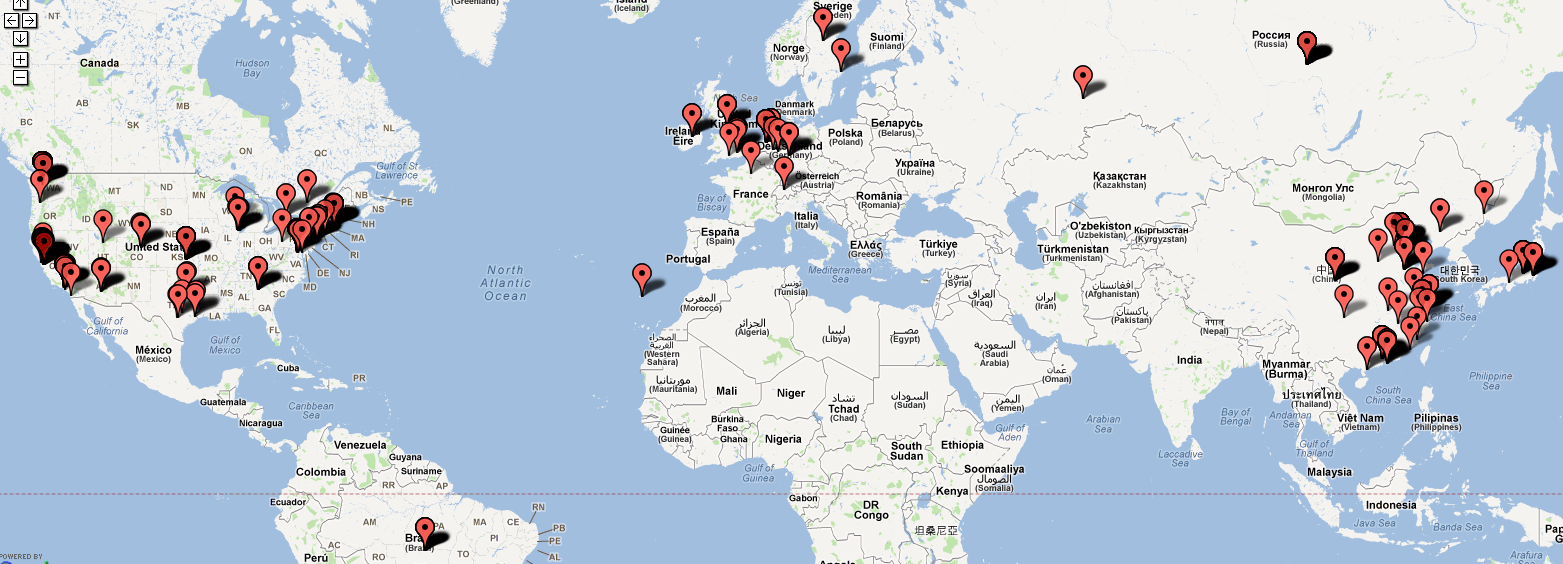
\includegraphics[keepaspectratio,width=\textwidth]{map}
\caption{Karta över positionen för de kontaktade servrarna}
\label{fig:gc}
\end{figure}

\end{document}
